%%%%%%%%%%%%%%%%%%%%%%%%%%%%%%%%%%%%%%%%%
% Large Colored Title Article
% LaTeX Template
% Version 1.1 (25/11/12)
%
% This template has been downloaded from:
% http://www.LaTeXTemplates.com
%
% Original author:
% Frits Wenneker (http://www.howtotex.com)
%
% License:
% CC BY-NC-SA 3.0 (http://creativecommons.org/licenses/by-nc-sa/3.0/)
%
%%%%%%%%%%%%%%%%%%%%%%%%%%%%%%%%%%%%%%%%%

%----------------------------------------------------------------------------------------
%	PACKAGES AND OTHER DOCUMENT CONFIGURATIONS
%----------------------------------------------------------------------------------------

%\documentclass[DIV=calc, paper=a4, fontsize=11pt, twocolumn]{scrartcl}	 
\documentclass[DIV=calc, paper=a4, fontsize=11pt]{scrartcl}	 % A4 paper and 11pt font size

\usepackage[english]{babel} % English language/hyphenation
\usepackage[protrusion=true,expansion=true]{microtype} % Better typography
\usepackage{amsmath,amsfonts,amsthm} % Math packages
\usepackage[svgnames]{xcolor} % Enabling colors by their 'svgnames'
\usepackage[hang, small,labelfont=bf,up,textfont=it,up]{caption} % Custom captions under/above floats in tables or figures
\usepackage{booktabs} % Horizontal rules in tables
\usepackage{fix-cm}	 % Custom font sizes - used for the initial letter in the document

\usepackage{sectsty} % Enables custom section titles
\allsectionsfont{\usefont{OT1}{phv}{b}{n}} % Change the font of all section commands

\usepackage{fancyhdr} % Needed to define custom headers/footers
\pagestyle{fancy} % Enables the custom headers/footers
\usepackage{lastpage} % Used to determine the number of pages in the document (for "Page X of Total")

\usepackage{listings}
\usepackage{upquote}
\usepackage[autolinebreaks,useliterate]{mcode}
\usepackage[margin=2.5cm]{geometry}
\usepackage{hyperref}
\usepackage{graphicx}
\usepackage{makeidx} 
\makeindex 

% Headers - all currently empty
%\textwidth
\fancyheadoffset{0cm}
\lhead{}
\chead{}
\rhead{}

% Footers
\lfoot{}
\cfoot{}
\rfoot{\footnotesize Page \thepage\ of \pageref{LastPage}} % "Page 1 of 2"

\renewcommand{\headrulewidth}{0.0pt} % No header rule
\renewcommand{\footrulewidth}{0.4pt} % Thin footer rule

\usepackage{lettrine} % Package to accentuate the first letter of the text
\newcommand{\initial}[1]{ % Defines the command and style for the first letter
\lettrine[lines=3,lhang=0.3,nindent=0em]{
\color{DarkGoldenrod}
{\textsf{#1}}}{}}

%----------------------------------------------------------------------------------------
%	TITLE SECTION
%----------------------------------------------------------------------------------------

\usepackage{titling} % Allows custom title configuration

\newcommand{\HorRule}{\color{DarkGoldenrod} \rule{\linewidth}{1pt}} % Defines the gold horizontal rule around the title

\pretitle{\vspace{-30pt} \begin{flushleft} \HorRule \fontsize{40}{40} \usefont{OT1}{phv}{b}{n} \color{DarkRed} \selectfont} % Horizontal rule before the title

\title{Maxtree Processing Toolbox} % Your article title

\posttitle{\par\end{flushleft}\vskip 0.5em} % Whitespace under the title

\preauthor{\begin{flushleft}\large \lineskip 0.5em \usefont{OT1}{phv}{b}{sl} \color{DarkRed}} % Author font configuration

\author{Philippe Salembier, Sergi Liesegang, } % Your name

\postauthor{\footnotesize \usefont{OT1}{phv}{m}{sl} \color{Black} % Configuration for the institution name
\\[1mm]Universitat Polit\`ecnica de Catalonia, BarcelonaTech \\
\url{https://imatge.upc.edu/}   % Your institution

\par\end{flushleft}\HorRule} % Horizontal rule after the title

\date{} % Add a date here if you would like one to appear underneath the title block

%----------------------------------------------------------------------------------------

\begin{document}

\maketitle % Print the title

\thispagestyle{fancy} % Enabling the custom headers/footers for the first page 

%----------------------------------------------------------------------------------------
%	ABSTRACT
%----------------------------------------------------------------------------------------

% The first character should be within \initial{}
\initial{T}\textbf{his document gives an overview of the Matlab Maxtree Processing Toolbox. The goal of this toolbox is to allow easy creation, processing and handling of Maxtree or Mintree representations. Many tools included in the toolbox are further discussed in~\cite{Salembier-TIP-2017}. The toolbox is useful to explore processing ideas and perform experiments on small size images. However, the toolbox has not been particularly optimized to minimize the CPU load nor the memory consumption. Therefore, if large size images have to processed, a proper optimized C/C++ implementation of the functions presented here should be used. }

%----------------------------------------------------------------------------------------
%	ARTICLE CONTENTS
%----------------------------------------------------------------------------------------
\tableofcontents

\section{Introduction}

Maxtree and Mintree are image (or signal) representations created by structuring the connected components resulting from  threshold decomposition~\cite{Salembier-Eusipco-1996,salembier_IEEEIP98}. They are also known as Component Trees~\cite{Jones-1997}. They provide a multiscale  description of extremas of images and signals and are, among other things, one of the classical ways to build connected operators~\cite{Salembier-IEEEIP-1995,Salembier-SPMag-2009}. Many algorithms to compute Maxtree from images have been proposed~\cite{Carlinet-IP-2014}.

In this Matlab toolbox, Maxtree/Mintrees are represented by a structure array with the following fields: 
\begin{lstlisting}[aboveskip=0.5 \baselineskip]
% Node:            	ID on the node in the tree (it is also the position 
%					of the node in the array)
% GrayLevel:       	Gray level of the pixels stored in the node
% Parent:          	ID of the Parent node
% Children:        	ID(s) of the Child node(s)
% NumberOfPixels	Number of pixels stored in the node
% Pixels			Offsets defining the pixel positions assuming that the 
%					array is stored in a vector form (column wise) 
\end{lstlisting}

%%%%%%%%%%%%%%%%%%%%%%%%%%%%%%%%%%%%%%%%%%%%%%%%%%
%%%%%%%%%%%%%%%%%%%%%%%%%%%%%%%%%%%%%%%%%%%%%%%%%%

\section{Installation}
The package involves standard \mcode{.m} Matlab functions plus a mex file. So just make sure that the toolbox folder is in Matlab path. To compile the mex file, simply run:

\begin{lstlisting}[aboveskip=0.5 \baselineskip]
mex maxtree_of_image.c
\end{lstlisting}
 
 A set of examples is provided in the \mcode{Examples.m} file. It illustrates basic tree creation and processing: \index{\mcode{Examples.m}}
 \begin{lstlisting}[aboveskip=0.5 \baselineskip]
%  Examples of function use of the maxtree Toolbox
%
%  Example 1: Simple maxtree construction, area filtering and image restitution 
%  Example 2: Maxtree construction, population with a random feature,
%             graph, tree and branch filtering of the feature, trees 
%             visualization with graphviz
%  Example 3: Extract the regional maxima of a feature on a tree and label them, 
%             tree visualization with graphviz
%  Example 4: Filter by reconstruction (Branch and Tree) applied on maxtree 
%             (markers are the absolute maxima of the feature), trees 
%             visualization with graphviz
%  Example 5: Compute a maxtree of a maxtree
%  Example 6: Compute a maxtree of a maxtree, AreaExtinction Filter the second 
%             maxtree to remove small maxima, Restore the filtered features in 
%             the first maxtree
%  Example 7: Visualization example: Construct a maxtree, visualization 
%             with maxtree_to_gv (Graphviz), branches_display and maxtree_plot 
%
\end{lstlisting}
 
%------------------------------------------------

%%%%%%%%%%%%%%%%%%%%%%%%%%%%%%%%%%%%%%%%%%%%%%%%%%
%%%%%%%%%%%%%%%%%%%%%%%%%%%%%%%%%%%%%%%%%%%%%%%%%%

\section{Creating Max/Mintrees}
Two set of functions are provided for the creation of Maxtree or Mintree.
\subsection{Tree creation from images}
The main function to create a Maxtree from a Matlab image is: \index{\mcode{maxtree_of_image.m}}
\begin{lstlisting}[aboveskip=0.5 \baselineskip]
%  Compute the maxtree of of an image
%
%		maxtree = maxtree_of_image(image, connectivity)
%
%  image should be an int16 array whose values are in [0,32000]
%  connectivity should be either 4 or 8 
\end{lstlisting}

\noindent The dual function creating Mintree is: \index{\mcode{mintree_of_image.m}}
\begin{lstlisting}[aboveskip=0.5 \baselineskip]
%  Compute the mintree of an image
%
%        mintree = mintree_of_image(image, connectivity)
%  
%  image should be an int16 array whose values are in [0,32000]
%  connectivity should be either 4 or 8 
\end{lstlisting}

\subsection{Tree creation from Maxtrees or Mintrees}
Maxtree and Mintrees can also be used to describe the connected components of any graph.
As Maxtrees and Mintrees are particular graphs, the connected components of a field \mcode{infield_name}
associated to nodes of a Maxtree or of a Mintree can be represented by a Maxtree or a Mintree~\cite{Xu-TPAMI-2015}: 
\index{\mcode{maxtree_of_maxmintree.m}}

\begin{lstlisting}[aboveskip=0.5 \baselineskip]
%  maxtree_of_maxmintree computes the maxtree of a maxtree or a mintree
%
%  maxtree_out = maxtree_of_maxmintree(tree, infield_name);
%
%  Input arguments:
%     tree:              	Structure for the maxtree or mintree
%     infield_name:         Field of the maxtree structure to analyze
%
%  Output argument:
%     maxtree_out:          Output maxtree describing the connected
%                           components of infield_name in tree
%
%  EXAMPLE
%     maxtree_out = maxtree_of_maxmintree(maxtree, 'Feature');
%
%  See also mintree_of_maxmintree
%
\end{lstlisting}

\noindent The dual representation, the Mintree, can be created with: \index{\mcode{mintree_of_maxmintree.m}}
\begin{lstlisting}[aboveskip=0.5 \baselineskip]
%  mintree_of_maxmintree computes the mintree of a maxtree or a mintree.
%
%  maxtree_out = mintree_of_maxmintree(tree, infield_name);
%
%  Input arguments:
%     tree:              	Structure for the maxtree or mintree
%     infield_name:         Field of the maxtree structure to analyze
%
%  Output argument:
%     maxtree_out:          Output mintree describing the connected
%                           components of infield_name in tree
%
%  EXAMPLE
%     maxtree_out = mintree_of_maxmintree(maxtree, 'Feature');
%
%  See also maxtree_of_maxmintree
%
\end{lstlisting}
%------------------------------------------------

%%%%%%%%%%%%%%%%%%%%%%%%%%%%%%%%%%%%%%%%%%%%%%%%%%
%%%%%%%%%%%%%%%%%%%%%%%%%%%%%%%%%%%%%%%%%%%%%%%%%%

\section{Creating Max/Mintree Attributes}
One of the major goals of this toolbox is to allow easy creation and processing of attributes in Maxtree or Mintree. These attributes defined on the tree structure can be considered as graph signals and processed with the corresponding graph signal processing tools. Populating each node of a Maxtree or a Mintree with an attribute value can be done with the following function: 
\index{\mcode{maxtree_Populate.m}}
\begin{lstlisting}[aboveskip=0.5 \baselineskip]
%  maxtree_populate populates a mintree or a maxtree with an attribute.
%
%  tree_out = maxtree_populate(tree, attribute);
%
%  Input arguments:
%     tree:                 Structure with the maxtree or mintree 
%     attribute:            Attribute to be computed. Available options: 
%                           'Area', 'MeanGrayLevel', 'Ellipse',
%                           'AreaExtinction', 'ContrastExtinction'
%  Optional arguments:
%     image:                In the case of the 'Ellipse' attribute an 
%                           image has to be passed to the function.
%  Output argument:
%     tree_out:             Output maxtree with the resulting attribute
%                           field
%  EXAMPLE
%     tree_out = maxtree_populate(tree, 'Area');
%     tree_out = maxtree_populate(tree, 'Ellispe', image);
%
\end{lstlisting}
This function makes a distinction between the pixels that are associated to a node and the connected components created by the threshold decomposition. The nodes in a Maxtree actually represent a structuring by inclusion of the connected components created by threshold decomposition. However, in order to minimize the memory requirement, the set of pixels actually assigned to a node are not the entire set of pixels belonging to the connected component, but only the subset that are at the same gray level value as the threshold. As a result, the set of pixels defining the connected component associated to a node can be obtained as the union of the pixels stored in a node and all its descendant nodes.
The features that are currently available include: 
\begin{itemize}
\item Area: Compute the number of pixels of the connected component associated to a current node. This number is equal to the sum of the number of pixels stored in the current node and all its descendant nodes.
\item MeanGrayLevel: Mean value of the \mcode{GrayLevel} field in the connected component (that is the area associated to the current node and all its descendant node). 
\item Ellipse: Each connected component associated to a node is approximated by an ellipse and Matlab region properties
`MajorAxisLength', `MinorAxisLength', `Orientation', `Eccentricity', `BoundingBox' are computed and associated with the node (this attribute relies on the Matlab \mcode{regionprops} command).
\item AreaExtinction:  Extinction attributes~\cite{Vachier-NSIP-1995} are useful to prune trees only at bifurcation 
points. They remove terminal branches which are complete sets of nodes going from a leaf node to a branch bifurcation. 
For an increasing attribute, the extinction value of a tree node is the maximal attribute value such that the terminal 
branch it belongs to still exists after the pruning. In the case of AreaExtinction, the attribute is the Area. 
\item ContrastExtinction:  This extinction attribute is similar to the previous one except that the criterion is the difference between the 
gray level value of a node and the maximum gray level value of the leaves among its descendant. 
\end{itemize}
This list of currently available features is rather limited. In practice, useful attributes are most of the time application dependant. Therefore the \mcode{maxtree_Populate} is provided as an example or a starting point that, hopefully, can be easily extended. 

\section{Max/Mintrees visualization}
Three functions are provided to visualize the content of a Maxtree or a Mintree. The first one relies on Graphviz (\url{http://www.graphviz.org/}) which is an open source graph visualization software. The Toolbox provides a function to export a Maxtree into a *.dot file that can be read and visualized by Graphviz. \index{\mcode{maxtree_to_gv.m}}

\begin{lstlisting}[aboveskip=0.5 \baselineskip]
%  maxtree_to_gv prints the Maxtree on a text file for vizualization with
%  graphviz. Graphviz is a package of open-source tools initiated by AT&T
%  Labs Research for drawing graphs specified in DOT language scripts. See:
%  http://www.graphviz.org
% 
%  maxtree_to_gv(filename, layout, maxtree);
%
%  Input arguments:
%     filename:             Name fo the file to store the .gv file 
%     layout:               Graphviz layout (preferably 'dot', 'sfdp', 'neato' 
%                           or 'twopi')
%     maxtree:              Maxtree structure
%
%  Optional arguments:
%     'Subtree',val,        Only the subtree rooted in node 'val' is displayed 
%                           (default 1)
%     'MaxNNodes',val,      Limit the number of nodes to be displayed to val
%                           (default all nodes are displayed)
%     'Attribute','name',   Name of the scalar field in the maxtree struct 
%                           to specify the gray level or color information 
%                           of the nodes (default 'GrayLevel')
%     'DisplayMode','name', Should be 'Color' or 'Gray' (default 'Gray') 
%     'Bounds',[min max],   Define the minimum and maximum values to be displayed 
% 
%  EXAMPLE
%       maxtree_to_gv(filename, 'dot', maxtree);
%       maxtree_to_gv(filename, 'sfdp', maxtree,'Subtree',15,'MaxNNodes',100,...
%           'Attribute','NumberOfPixels','DisplayMode','Color','Bounds',[0 10]);
%

\end{lstlisting}
The function has three mandatory arguments plus a set of optional arguments. By default, the nodes displayed by Graphviz are filled with a gray level value representing the   values in the field \mcode{maxtree(:).GrayLevel}, but the `Attribute' argument can be used to change this behavior. If `Bounds' is not specified the values are scaled so that they are visualized from black (lowest value) to white (highest value). Note that these values can also be visualized in color (from the lowest value in blue to the highest value in red).  

This first visualization strategy is useful to analyze the tree structure or the values of features on specific nodes but it is not appropriate to handle very large trees nor to study the evolution of a feature along the tree branches. This is the reason why a second visualization option is provided. It involves two functions \mcode{maxtree_to_branches} and \mcode{branches_display}. The idea illustrated in Fig.~\ref{fig:visualization} is to create an image, called ``branch image", where each tree branch is represented by a column and the gray level evolution along the image columns describe the evolution of the feature along the tree branches. Note that the information of some nodes are duplicated in this representation. For example, the root node belongs to all tree branches. This root node is represented by the bottom line of the branch image. So all the pixels of this bottom line have the same gray level values. The height of the branch image is defined by the length of the longest branch. As seen in Fig.~\ref{fig:visualization}, the various branches start with the root node at the bottom of the image and ends at different position depending on their length. The branch image pixels above the end of a branch are represented by default by a zero value (but this can be changed with the \mcode{AboveTreeValue} argument). 
\begin{figure}[t]
\centering
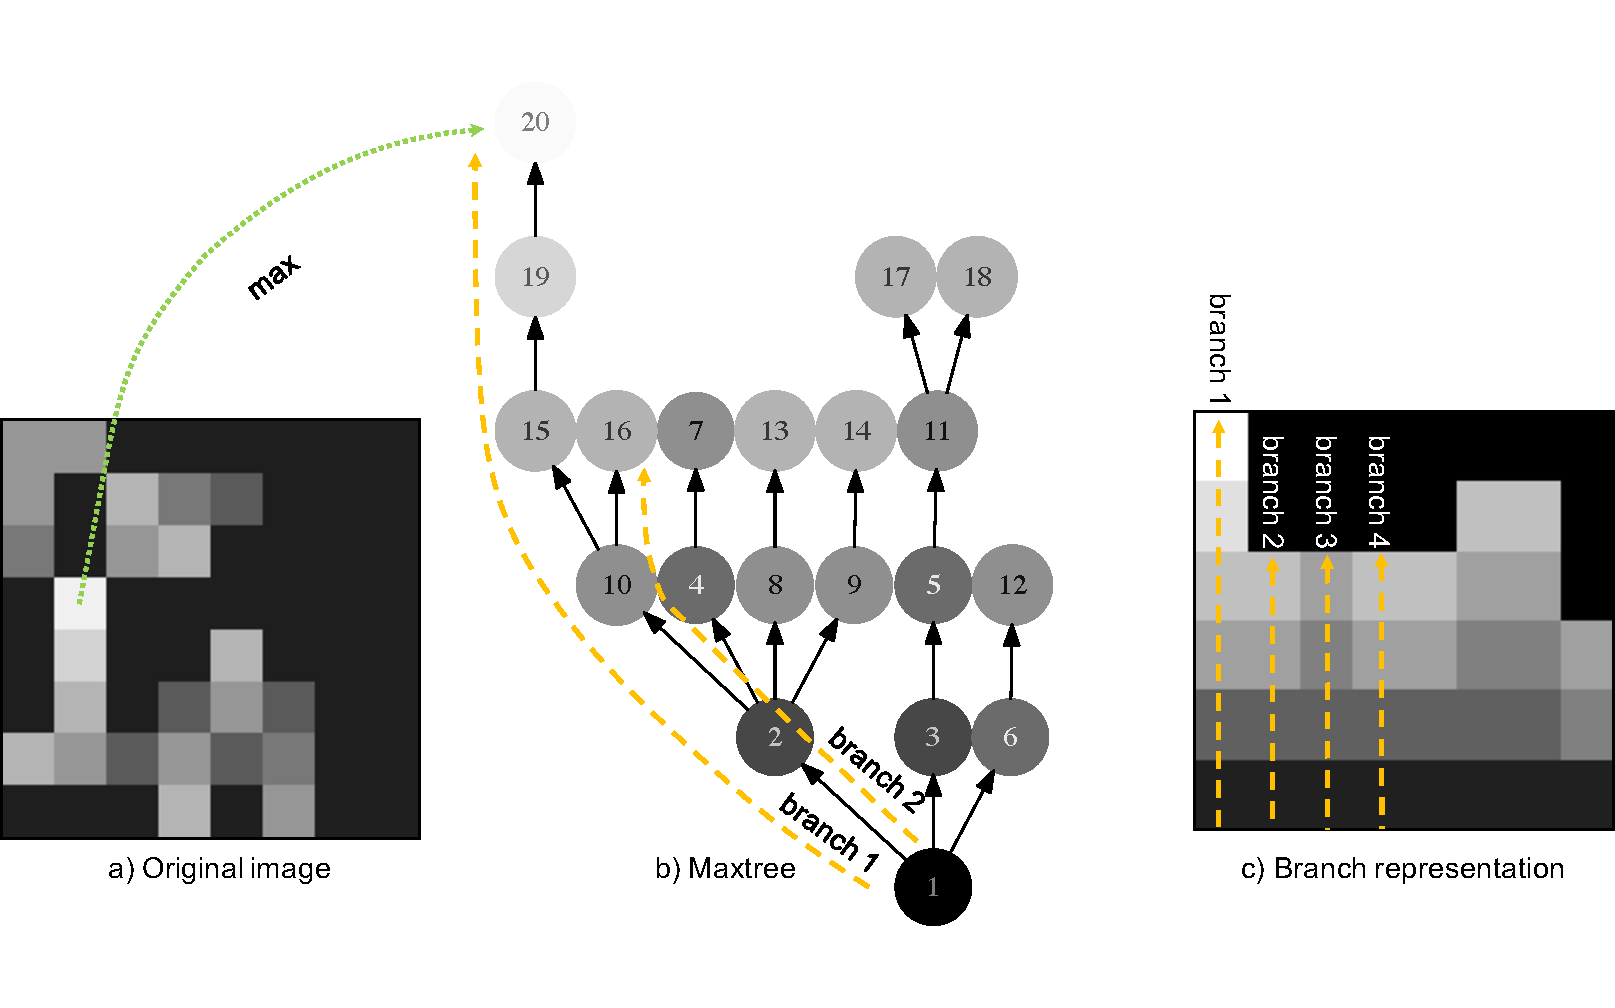
\includegraphics[width=10cm]{Fig/Visualization.pdf}  
\caption{Illustration of branch visualization. Left: Original image, Center: Maxtree of the original image (the gray level of the nodes represents the gray level values of the original image pixels). Right: Image representing the evolution of a feature (here the node gray level value) along the branches.}
\label{fig:visualization}
\end{figure}

In order to generate this representation, the first step is to create an image defining the mapping between the Maxtree or Mintree nodes and the branch image. This is done by the following function: \index{\mcode{maxtree_to_branches.m}}

\begin{lstlisting}[aboveskip=0.5 \baselineskip]
%  maxtree_to_branches creates a "branches" map from a maxtree or mintree 
%  The branch map is an image where the pixel graylevel value indicates 
%  the node ID in the tree. The function will also change the order
%  of the children of each node so that they are in decreasing order of 
%  branch length. This allows a better visualization. The function output
%  is the branch map and the tree with the reordered children. 
% 
%  [branches, tree] = maxtree_to_branches (tree);
%
%  Input arguments:
%     tree:              Structure with the maxtree or mintree 
%
%  Output arguments:
%     branches:          Branch map image
%     tree:              Input tree where children are ordered as a
%                        function of the branch length
%  EXAMPLE
%     [branches, tree] = maxtree_to_branches (tree);
%
%  See also maxtree_branches_display
%
\end{lstlisting}
Note that this function outputs the branch map \mcode{branches} and also a slightly modified version of the tree. Indeed, it has been observed that it is easier to interpret the branch images when the branches are organized as a function of their length. As a result, the \mcode{maxtree_to_branches} re-orders the children of each node such that the children corresponding to the longest branches appear first in the list of children nodes. This reordering of children has also an impact on the visualization with Graphviz. So, if one wants to compare the Graphviz visualization with the branch image visualization, it is recommended to call both \mcode{maxtree_to_gv} and \mcode{maxtree_branches_display} after calling \mcode{maxtree_to_branches}.

Once the \mcode{maxtree_to_branches} has been called, the visualization of a particular feature can be done with: 
\index{\mcode{maxtree_branches_display.m}}
\begin{lstlisting}[aboveskip=0.5 \baselineskip]
%  maxtree_branches_display displays a maxtree field as an image following
%  the branch mapping.
%
%  image = maxtree_branches_display(maxtree, branches, field_name);
%
%  Input arguments:
%     maxtree:              Maxtree or mintree structure
%     branches:             Branches mapping created by maxtree_to_branches
%     field_name:           Field to be displayed
%  Optional arguments:
%     'AboveTreeValue',val, Value of the upper part of the image that does
%                           not correspond to actual nodes (default 0)
%  Output argument:        
%     image:                Image describing the evolution of field_name
%                           values along the tree branches
%
%  EXAMPLE 
%     image = maxtree_branches_display(maxtree, branches, field_name);
%
%  See also maxtree_to_branches
%
\end{lstlisting}

Finally, a third visualization function is provided to plot the evolution of a feature from a given node to the root node. 
\index{\mcode{maxtree_plot.m}}
\begin{lstlisting}[aboveskip=0.5 \baselineskip]
%  maxtree_plot plots the field_name values of a Maxtree from the node
%  "node" to the root.
%
%  maxtree_plot(maxtree, node, field_name);
%
%  Input arguments:
%     maxtree:              Maxtree structure
%     node:                 Id of the node to start the plot (the plot goes
%                           up to the root node)
%     field_name:           Field to be displayed
%     varargin:             Plot option of the type '-r', '--b', etc. 
%
%  EXAMPLE
%     maxtree_plot(maxtree, 10, 'GrayLevel', '-r');
%
%  See also maxtree_to_branches, branches_display
%
\end{lstlisting}



%%%%%%%%%%%%%%%%%%%%%%%%%%%%%%%%%%%%%%%%%%%%%%%%%%
%%%%%%%%%%%%%%%%%%%%%%%%%%%%%%%%%%%%%%%%%%%%%%%%%%

\section{Processing Max/Mintrees}

\subsection{Pruning}
One of the initial motivations to define Maxtree and Mintree was to create connected operators~\cite{Salembier-IEEEIP-1995,Salembier-SPMag-2009}. The strategy consists in creating a Maxtree or Mintree representation of an image, to populate it with an attribute and then to prune the tree. The pruning implemented in this toolbox is a simple node pruning that compares the node attribute value to a threshold: 
\index{\mcode{maxtree_Prune.m}}
\begin{lstlisting}[aboveskip=0.5 \baselineskip]
%  maxtree_Prune prunes a mintree or a maxtree based on some attribute
%  values
%
%  tree_out = maxtree_Prune(tree, attribute, threshold, decision);
%
%  Input arguments:
%     maxtree:              Structure with the maxtree or mintree 
%     attribute:            Attribute on which the pruning is defined
%     threshold:            Value of the threshold on the attribute 
%     decision:             Type of decision: 'Direct, 'Min', 'Max' or
%                           'Subtract'
%  Output argument:
%     tree_out:             Output pruned tree 
%
%  EXAMPLE
%     maxtree_out = maxtree_Prune(maxtree, 'Area', 10, 'Direct');
%
\end{lstlisting}
The choice of a proper decision rule is important in the case of non-increasing attribute: 
\begin{itemize}
\item The {\em Max} rule prunes the branches from the leaves up to the first node that has to be preserved.
\item The {\em Min} rule prunes the branches from the leaves up to the last node that has to be removed.
\item The {\em Direct} rule consists of simply removing the nodes that have to be removed even if this does not create a pruning strategy. The pixels belonging to the nodes that have been removed are merged to the node of their first ancestor that has to be preserved.
\item The {\em Subtractive} rule is the same as the direct rule except that the gray levels of surviving descendants of removed nodes are also lowered, so that the contrast with the local background remains the same.
\end{itemize}

\subsection{Filters}
Maxtree and Mintree are special cases of graphs and the notion of graph processing tools apply to them. Now, the fact that Maxtree and Mintree are hierarchical structure where, depending on the application, the connectivity from a Node towards its Parent or towards its Children may not be equivalent, several notions of filtering can be defined. Three different filtering notions are defined in this package: ``Graph filter'', ``Tree filter'' and ``Branch filter''. To explain the difference between these three notions, let us consider for example the ``Mean'' filter of size 2 applied on the Maxtree of Fig.~\ref{fig:visualization}. Assume we are processing node number 8. 
\begin{itemize}
\item Graph Filter: The ``Graph mean value'' of size 2 is the mean value of all nodes which are at distance lower or equal to 2 in the graph. In the case of node 10, this corresponds to the mean value of nodes: 10, 2, 15, 16, 1, 4, 8, 9, 19 (nodes 2, 15, 16 are at distance 1 and nodes 1, 4, 8, 9, 19 at distance 2). 
\item Tree Filter: The ``Tree mean value'' of size 2 is the mean value of all \underline{ancestor nodes} and \underline{descendant nodes} of the current node which are at distance lower or equal to 2. In the case of node 10, this corresponds to the mean value of nodes: 10, 2, 15, 16, 1, 19 (nodes 2 and 1 are the ancestors at distance lower or equal to 2. Nodes 15 and 16 are descendants at distance 1 and nodes 10 is a descendant at distance 2). 
\item Branch Filter: The ``Branch mean'' considers all the individual branches to which the current node belongs. Node 8 belongs to two different branches: 20-19-15-10-2-1 and 16-10-2-1. Therefore, two mean values are computed in what is called the {\em estimation step}: $m_1=mean(node_{20},node_{19},node_{15},node_{10},node_{2},node_{1})$ and $m_2=mean(node_{16},node_{10},node_{2},node_{1})$. Then, the final result is the aggregation of the individual $m_i$ mean values: $m=mean(m_1,m_2)$. 
\end{itemize}

In this toolbox, three functions are related to these three filtering notions. The Graph Filters are defined in: \index{\mcode{maxtree_GFilter.m}}
\begin{lstlisting}[aboveskip=0.5 \baselineskip]
%  maxtree_GFilter computes a Graph Filter on attributes of Maxtrees. In
%  Graph filters, the neigborhood is defined on the basis of the graph
%  connectivity
%
%  maxtree_out = maxtree_GFilter(maxtree, filter, parameter, infield_name, outfield_name);
% 
%  Input arguments:
%     maxtree:              Maxtree structure
%     filter:               Type of filters, possible values are: 
%                           'Erosion','Dilation',
%                           'Opening','Closing',
%                           'Mean','Median'
%     parameter:            Size of the neighborhood in the graph
%     infield_name:         Name of the field defining the input data
%     outfield_name:        Name of the field defining the output data
% 
%  Output argument:
%     maxtree_out:          Output maxtree with the resulting outfield_name
%                           field
%  EXAMPLE 
%     maxtree = maxtree_GFilter(maxtree,'Opening',2,'GrayLevel','Out');
%
%  See also maxtree_TFilter, maxtree_BFilter, maxtree_BFilter2
%
\end{lstlisting}

The Tree Filters are defined in: 
\index{\mcode{maxtree_TFilter.m}}
\begin{lstlisting}[aboveskip=0.5 \baselineskip]
%  maxtree_TFilter computes a Tree Filter on attributes of Maxtrees. In
%  Tree filters, the neigborhood does not include the siblings of the node
%  to be filtered nor their descendants. 
%
%  maxtree_out = maxtree_TFilter(maxtree, filter, parameter, infield_name, outfield_name);
%
%  Input arguments:
%     maxtree:              Maxtree structure
%     filter:               Type of filters, possible values are: 
%                           'Erosion','Dilation',
%                           'Opening','Closing',
%                           'Mean','Median'
%     parameter:            size of the neighborhood in the branch
%     infield_name:         Name of the field defining the input data
%     outfield_name:        Name of the field defining the output data
% 
%  Output argument:
%     maxtree_out:          Output maxtree with the resulting outfield_name
%                           field
%  EXAMPLE 
%     maxtree = maxtree_TFilter(maxtree,'Opening',2,'GrayLevel','Out');
%
%  See also maxtree_GFilter, maxtree_BFilter, maxtree_BFilter2
%
\end{lstlisting}

Finally, the Branch Filters are defined in: 
\index{\mcode{maxtree_BFilter.m}}
\begin{lstlisting}[aboveskip=0.5 \baselineskip]
%  maxtree_BFilter computes a Branch Filter on attributes of Maxtrees. In
%  Branch filters, each branch is individually filtered (estimation step)
%  and then the resulting estimated values are aggregated.
%
%  maxtree_out = maxtree_BFilter(maxtree, filter, parameter, aggregation,...
%                infield_name, outfield_name);
%
%  Input arguments:
%     maxtree:              Maxtree structure
%     filter:               Type of (estimation) filters, possible values are: 
%                           'Erosion','Dilation', 'Mean','Median'
%     parameter:            Size of the neighborhood in the branch
%     aggregation:          Type of aggregation, possible values are:
%                           'Mean','Median', 'Max', 'Min''
%     infield_name:         Name of the field defining the input data
%     outfield_name:        Name of the field defining the output data
%
%  Output argument:
%     maxtree_out:          Output maxtree with the resulting outfield_name
%                           field
%  EXAMPLE 
%     maxtree = maxtree_BFilter(maxtree,'Opening',2,'Median','GrayLevel','Out');
%
%  See also maxtree_GFilter, maxtree_TFilter, maxtree_BFilter2
%
\end{lstlisting}
Note that in this last case, two filters have to be defined: one for the estimation step and one for the aggregation step. The toolbox also
includes an alternative version of this function that is more efficient for large values of \mcode{parameter}. \index{\mcode{maxtree_BFilter2.m}}
\begin{lstlisting}[aboveskip=0.5 \baselineskip]
%  maxtree_BFilter2 computes a Branch Filter on attributes of Maxtrees. In
%  Branch filters, each branch is individually filtered (estimation step)
%  and then the resulting estimated values are aggregated. This function is
%  an alternative implementation of maxtree_BFilter. It is faster in
%  particular for large values of the 'parameter' (Note that the padding
%  strategy is slightly different in both functions. So the results are
%  slightly different). 
% 
%  maxtree_out = maxtree_BFilter2(maxtree, branches, filter, parameter,... 
%                aggregation, infield_name, outfield_name);
%
%  Input arguments:
%     maxtree:              Maxtree structure
%     branches:             Branch representation of the maxtree computed 
%                           with maxtree_to_branches
%     filter:               Type of (estimation) filter, possible values are: 
%                           'Erosion','Dilation', 'Mean','Median'
%     parameter:            size of the neighborhood in the branch
%     aggregation:          Type of aggregation, possible values are:
%                           'Mean','Median', 'Max', 'Min''
%     infield_name:         Name of the field defining the input data
%     outfield_name:        Name of the field defining the output data
%
%  Output argument:
%     maxtree_out:          Output maxtree with the resulting outfield_name
%                           field
%  EXAMPLE 
%     maxtree = maxtree_BFilter2(maxtree,branches,'Opening',2,'Median','GrayLevel','Out');
%
%  See also maxtree_to_branches, maxtree_GFilter, maxtree_TFilter, maxtree_BFilter
%
\end{lstlisting}

\subsection{Morphological reconstruction}
Morphological reconstruction propagates by dilation a marker signal while forcing it to remain below a reference signal. 
The Matlab \mcode{imreconstruct} function performs this reconstruction in the case of images. In this toolbox, 
two different notions of reconstruction for Maxtrees are available: ``Graph reconstruction'' and ``Tree reconstruction''.
\begin{itemize}
\item Graph reconstruction: The propagation involved in the reconstruction is done following the graph connectivity. 
\item Tree reconstruction: The propagation involved in the reconstruction is limited to a 1D propagation: either from the root to the leaves 
or from the leaves to the root. It is more limited than the Graph reconstruction.  
\end{itemize}

The following function performs the graph reconstruction: 
\index{\mcode{maxtree_GReconstruct.m}}
\begin{lstlisting}[aboveskip=0.5 \baselineskip]
% maxtree_GReconstruct computes the morphological reconstruction of
% mar_field_name with reference to ref_field_name in a maxtree.  The
% reconstruction process uses the Graph connectivity defined by the tree.
%
% maxtree_out =  maxtree_GReconstruct(maxtree, ref_field_name, mar_field_name, outfield_name);
%
%  Input arguments:
%     maxtree:              Maxtree structure
%     ref_field_name:       Name of the field to be used as reference 
%     mar_field_name:       Name of the field to be used as marker 
%     outfield_name:        Name of the output field  
%
%  Output argument:
%     maxtree_out:          Output maxtree with the resulting outfield_name
%                           field
%  EXAMPLE 
%       maxtree = maxtree_GReconstruct(maxtree, 'Graylevel', 'Marker', 'Out');
%
%  See also maxtree_GDualReconstruct
%
\end{lstlisting}
The tree reconstruction is implemented in: 
\index{\mcode{maxtree_TReconstruct.m}}
\begin{lstlisting}[aboveskip=0.5 \baselineskip]
%  maxtree_TReconstruct computes the morphological Tree reconstruction of
%  mar_field_name with reference to ref_field_name in a maxtree. The
%  reconstruction process is either 'Root_to_Leaves' or 'Leaves_to_Root'.
%
%  maxtree_out =  maxtree_TReconstruct(maxtree, type, ref_field_name, mar_field_name, outfield_name);
%
%  Input arguments:
%     maxtree:              Maxtree structure
%     type:                 Type of reconstruction: 'Root_to_Leaves' or
%                           'Leaves_to_Root'.
%     ref_field_name:       Name of the field to be used as reference 
%     mar_field_name:       Name of the field to be used as marker 
%     outfield_name:        Name of the output field  
%
%  Output argument:
%     maxtree_out:          Output maxtree with the resulting outfield_name
%                           field
%  EXAMPLE 
%       maxtree = maxtree_TReconstruct(maxtree, 'Root_to_Leaves', 'Graylevel', 'Marker', 'Out');
%
%  See also maxtree_TDualReconstruct
%
\end{lstlisting}

As classically done in Mathematical Morphology, the dual reconstructions can also be defined. They propagate by erosion a marker signal while forcing it to remain above a reference signal. In the Maxtree/Mintree cases, two functions are defined. For the graph reconstruction:
\index{\mcode{maxtree_GDualReconstruct.m}}
\begin{lstlisting}[aboveskip=0.5 \baselineskip]
%  maxtree_GDualReconstruct computes the dual morphological reconstruction
%  of mar_field_name with reference to ref_field_name in a maxtree. The
%  reconstruction process uses the Graph connectivity defined by the tree.
%
%  maxtree_out =  maxtree_GDualReconstruct(maxtree, ref_field_name, mar_field_name, outfield_name);
% 
%  Input arguments:
%     maxtree:              Maxtree structure
%     ref_field_name:       Name of the field to be used as reference 
%     mar_field_name:       Name of the field to be used as marker 
%     outfield_name:        Name of the output field  
%
%  Output argument:
%     maxtree_out:          Output maxtree with the outfield_name field
%
%  EXAMPLE 
%     maxtree = maxtree_GDualReconstruct(maxtree, 'Graylevel', 'Marker', 'Out');
%
%  See also maxtree_GReconstruct
%
\end{lstlisting}
And for the tree reconstruction: 
\index{\mcode{maxtree_TDualReconstruct.m}}
\begin{lstlisting}[aboveskip=0.5 \baselineskip]
%  maxtree_TDualReconstruct computes the dual morphological Tree
%  reconstruction of mar_field_name with reference to ref_field_name in a
%  maxtree. The reconstruction process is either 'Root_to_Leaves' or
%  'Leaves_to_Root'. 
%
%  maxtree_out =  maxtree_TDualReconstruct(maxtree, type, ref_field_name, ...
%                 mar_field_name, outfield_name);
%
%  Input arguments:
%     maxtree:              Maxtree structure
%     type:                 Type of reconstruction: 'Root_to_Leaves' or 
%                           'Leaves_to_Root'.
%     ref_field_name:       Name of the field to be used as reference 
%     mar_field_name:       Name of the field to be used as marker 
%     outfield_name:        Name of the output field  
%
%  Output argument:
%     maxtree_out:          Output maxtree with the resulting outfield_name
%                           field
%  EXAMPLE 
%       maxtree = maxtree_TDualReconstruct(maxtree, 'Root_to_Leaves', ...
%                 'Graylevel', 'Marker', 'Out');
%
%  See also maxtree_TReconstruct
%
\end{lstlisting}

\subsection{Other processing functions}
Regional extrema on a Maxtree or a Mintree can be identified with the following function:
\index{\mcode{maxtree_RegExtrema.m}}
\begin{lstlisting}[aboveskip=0.5 \baselineskip]
%  maxtree_RegExtrema identifies regional extrema of attributes on maxtrees
%  or mintrees
%
%  maxtree_out = maxtree_RegExtrema(maxtree, extrema, infield_name, outfield_name);
%
%  Input arguments:
%     maxtree:              Maxtree structure
%     extrema:              'Min' or 'Max'
%     infield_name:         Field of the maxtree structure on which to
%                           compute the extremas
%     outfield_name:        Field to define the position of the extremas
%                           Min/Max = 1, otherwise 0
%  Output argument:
%     maxtree_out:          Output maxtree with the resulting outfield_name
%                           field
%  EXAMPLE
%     maxtree_out = maxtree_RegExtrema(maxtree, 'Min', 'GrayLevel', 'Marker');
%
\end{lstlisting}
Note that the extrema are defined following the Graph connectivity. 

Connected components (following the Graph connectivity) of a binary field can be labeled with the following function: 
\index{\mcode{maxtree_Label.m}}
\begin{lstlisting}[aboveskip=0.5 \baselineskip]
%  maxtree_Label assigns a different label to all connected components that
%  are different from 0.
%
%  maxtree_out = maxtree_Label(maxtree, infield_name, outfield_name);
%
%   Input arguments:
%     maxtree:              Maxtree structure
%     infield_name:         Field of the maxtree structure to label
%     outfield_name:        Field to output the labels
%
%   Output argument:
%     maxtree_out:          Output maxtree with the resulting outfield_name
%                           field
%  EXAMPLE 
%       maxtree = maxtree_Label(maxtree, infield_name, outfield_name));
%
\end{lstlisting}

%%%%%%%%%%%%%%%%%%%%%%%%%%%%%%%%%%%%%%%%%%%%%%%%%%
%%%%%%%%%%%%%%%%%%%%%%%%%%%%%%%%%%%%%%%%%%%%%%%%%%

\section{Image or tree restitution}
A Maxtree or a Mintree represents an image (or a signal) or a Maxtree/Mintree. Once it has been processed or pruned, it can be used to generate an image or Maxtree/Mintree. This is the restitution step. When a Maxtree or Mintree represents an image, the restitution can be done with: 
\index{\mcode{image_Restitution.m}}
\begin{lstlisting}[aboveskip=0.5 \baselineskip]
%  image_Restitution restores an image from a mintree or a maxtree.
%
%  image = image_Restitution(tree, field, width, height);
%
%  Input arguments:
%     tree:              Structure with the maxtree or mintree 
%     field_name:        name of the field to create the image
%     width:             width of the image
%     height:            height of the image
%
%  Output argument:
%     image:             Output image 
% 
%  EXAMPLE 
%     ima = image_Restitution(tree, 'GrayLevel', 256, 256);
%
%  See also tree_Restitution
%
\end{lstlisting}

If the Maxtree or Mintree represents a Maxtree or a Mintree, the restitution can be done with: 
\index{\mcode{tree_Restitution.m}}
\begin{lstlisting}[aboveskip=0.5 \baselineskip]
%  tree_Restitution restitutes a tree field from a mintree or a maxtree 
%
%  tree_out = tree_Restitution(tree2, field2, tree1, field1);
%
%  Input arguments:
%     tree2:            Structure with the maxtree (or mintree) of the maxtree (or mintree) 
%     field2:           Name of the field of tree2 to restitute the tree1
%                       (likely to be 'GrayLevel')
%     tree1:            Structure with the maxtree (or mintree) defining 
%                       the connectivity for the restitution 
%     field1:           Name of the field of tree1 to store the restitution
%
%  Output argument:
%     tree_out:         Output tree1 with the added field1 
%
%  EXAMPLES
%       tree_out = tree_Restitution(tree2, 'GrayLevel', tree1, 'GrayLevel_Processed');
%
%  See also image_Restitution
% 
\end{lstlisting}

%----------------------------------------------------------------------------------------
%	REFERENCE LIST
%----------------------------------------------------------------------------------------
%\bibliographystyle{unsrt}
%\bibliography{biblio_philippe}

\begin{thebibliography}{1}

\bibitem{Salembier-TIP-2017}
P.~Salembier, S.~Liesegang, and C.~L\'opez-Mart\'inez,
\newblock Ship Detection in SAR Images based on Maxtree Representation and Graph Signal Processing
\newblock {\em IEEE Transactions on Geoscience and Remote Sensing}, Accepted for publication, 2018.
  
 \bibitem{Salembier-Eusipco-1996}
P.~Salembier, A.~Oliveras, and L.~Garrido.
\newblock Motion connected operators for image sequences.
\newblock In {\em VIII European Signal Processing Conference, EUSIPCO'96},
  pages 1083--1086, Trieste, Italy, September 1996.

\bibitem{salembier_IEEEIP98}
P.~Salembier, A.~Oliveras, and L.~Garrido.
\newblock Anti-extensive connected operators for image and sequence processing.
\newblock {\em IEEE Transactions on Image Processing}, 7(4):555--570, April
  1998.

\bibitem{Jones-1997}
R.~Jones.
\newblock Component trees for image filtering and segmentation.
\newblock In {\em 1997 IEEE Workshop on Nonlinear Signal and Image Processing},
  Mackinac Island, USA, 1997.

\bibitem{Salembier-IEEEIP-1995}
P.~Salembier and J.~Serra.
\newblock Flat zones filtering, connected operators, and filters by
  reconstruction.
\newblock {\em IEEE Transactions on Image Processing}, 4(8):1153--1160, 1995.

\bibitem{Salembier-SPMag-2009}
P.~Salembier and M.~H.~F. Wilkinson.
\newblock Connected operators: A review of region-based morphological image
  processing techniques.
\newblock {\em IEEE Signal Processing Magazine}, 6:136--157, 2009.

\bibitem{Carlinet-IP-2014}
E.~Carlinet and T.~G{\'e}raud.
\newblock A comparative review of component tree computation algorithms.
\newblock {\em IEEE Transactions on Image Processing}, 23(9):3885 -- 3895,
  2014.

\bibitem{Xu-TPAMI-2015}
Y.~Xu, T.~Geraud, and L.~Najman.
\newblock Connected filtering on tree-based shape-spaces.
\newblock {\em IEEE Transactions on Pattern Analysis and Machine Intelligence},
  2015.

\bibitem{Vachier-NSIP-1995}
C.~Vachier and F.~Meyer.
\newblock Extinction value: a new measurement of persistence.
\newblock In {\em IEEE Workshop on Nonlinear Signal and Image Processing},
  volume~I, pages 254--257, 1995.

\end{thebibliography}


%----------------------------------------------------------------------------------------

\printindex 

\end{document}